\documentclass[parskip=full]{scrartcl}
\usepackage[utf8]{inputenc} % use utf8 file encoding for TeX sources
\usepackage[T1]{fontenc}    % avoid garbled Unicode text in pdf
\usepackage[german]{babel}  % german hyphenation, quotes, etc
\usepackage{hyperref}       % detailed hyperlink/pdf configuration
\hypersetup{                % ‘texdoc hyperref‘ for options
pdftitle={SWT1: Lastenheftvorlage},%
bookmarks=true,%
}
\usepackage{graphicx}       % provides commands for including figures
\usepackage{csquotes}       % provides \enquote{} macro for "quotes"
\usepackage[nonumberlist]{glossaries}     % provides glossary commands
\usepackage{enumitem}

\makenoidxglossaries
%
% % Glossareinträge
%
\newglossaryentry{Nutzer}
{
	name=Nutzer,
	plural=Nutzer,
	description={(Zahlende) Person welche die Dienste der Applikation nutzt},
}

\newglossaryentry{Abonnament}
{
	name=Abonnament,
	plural=Abonnaments,
	description={Zahlungssystem bei dem der Nutzer monatlich einen festen Betrag zahlt}
}

\newglossaryentry{HDR-Bild}
{
	name=HDR-Bild,
	plural=HDR-Bilder,
	description={(High Dynamic Range Image) Eine Rastergrafik, die große Helligkeitsunterschiede detailreich wiedergibt}
}

\newglossaryentry{Smartphone}
{
	name=Smartphone,
	description={Mobiltelefon mit Touchscreen und zusätzlichen Funktionen wie GPS und der Möglichkeit, Apps darauf zu installieren}
}

\title{iMage Lastenheft}
\author{Simon Himmel, 2210373}

\begin{document}

\maketitle

%
% % Hinweise - sollen nicht im endgültigen Dokument erscheinen, daher vor der Abgabe löschen!
%
\section{Vorwort}
Die Dokumentation der Pakete ist häufig lesenswert.
Insbesondere bei den Paketen hyperref und scrguide (KOMA-Script).
Wer TeXLivei per Kommandozeile benutzt kann einfach texdoc scrguide aufrufen.
Windows-Benutzer, die noch nie mit Latex gearbeitet haben, können sich alternativ MikTex anschauen; Mac-Benutzer MacTex.

Zum Erzeugen eines PDFs aus den LATEX-Sourcen empfehlen wir einen Wrapper wie latexmk\footnote{\url{https://www.ctan.org/tex-archive/support/latexmk}} oder einen Editor wie TeXStudio\footnote{\url{http://www.texstudio.org/}} zu verwenden.
Dieser übernimmt beispielsweise das mehrfache Ausführen von pdflatex, wo es notwendig ist.

Legen Sie für dieses Dokument ein neues Verzeichnis in Ihrem Git an, zum Beispiel \texttt{image.lastenheft} und speichern Sie alle benötigten Dateien darin.
Speichern Sie keine von Latex generierten Dateien (außer dem PDF) im Git.
Dies geschieht über die mitgelieferte \texttt{.gitignore}.
Sie können aber auch Ihre persönliche \texttt{.gitignore} bei Bedarf erweitern.

\section{Technisches Schreiben}

Technisches Schreiben ist wichtig für alle Arten von technischen und wissenschaftlichen Dokumenten, also auch im PSE und in der Bachelorarbeit.
Es bedeutet vor allem eine präzise Ausdrucksweise und widerspricht dabei einigen Regeln, die man im Deutschunterricht gelernt hat.
Ein paar praktische Tipps (aus den PSE-Dokumenten von Prof. Snelting):
\begin{itemize}[nosep]
\item Vermeide Adjektive.
      Oft (nicht immer) sind sie unnötig oder ein schlechter Ersatz für einen ungenauen Begriff.
\item Nebensatzkonstruktionen vermeiden; Hauptsätze verwenden!
\item Definiere Begriffe klar und verwende keine Synonyme.
      Synonyme lassen offen, ob genau das gleiche gemeint ist oder nur etwas ähnliches.
      Definiere spezielle Begriffe, z.B. \gls{Computer}, in einem Glossar und verweise im Dokument entsprechend darauf.
\item Abkürzungen sollten bei der ersten Verwendung (EV) ausgeschrieben werden.
      Nach der EV reicht dann die Kurzform.
\item Versuche konkrete Zahlen und Namen anzugeben.
      Vermeide ungenaue Ausflüchte wie: meistens, viele, oft, möglichst, üblich, jemand, manche.
\item Viele kurze Sätze sind einfacher zu verstehen als wenige lange Sätze.
\item Beispiele machen das Endprodukt greifbarer.
\item Illustrationen minimalistisch halten (z.B. IKEA Bauanleitung).
      Eine Information, ein Bild.
      Lieber mehrere ähnliche Bilder als ein komplexes Bild.
\item Vermeide Wiederholung, stattdessen Referenzen benutzen.
      Wiederholungen haben oft subtile Unterschiede, was zu Unklarheit und Verwirrung führt.
      Bei Änderungen wird oft vergessen, dass Wiederholungen auch angepasst werden müssen.
\item Versionskontrolle ergibt auch für technische Texte Sinn und nicht nur für Code.
\end{itemize}

%
% % Hier beginnt die Gliederung des Lastenhefts
%
\section{Zielbestimmung}
Der Benutzer soll durch das Produkt in die Lage versetzt werden, aus seinen eigenen Aufnahmen, gegen bezahlung, HDR-Bilder zu erstellen.

\section{Produkteinsatz}
Das Produkt dient zur erstellung von HDR-Bildern gegen bezahlung. Außerdem sollen diese auch auf sozialen Netzwerken hochgeladen werden können.

Zielgruppe: jeder Nutzer der Applikation.

Plattform: Smartphones mit IOS oder Android Betriebssystem.

\section{Funktionale Anforderungen}
\begin{itemize}[nosep]
\item[FA10] Ersterfassung, Änderung und Löschung von Nutzern (deren Konten).
\item[FA20] Erstellen und Speichern eines HDR-Bildes aus einer Bilderreihe der größe 3.
\item[FA30] Möglichkeit zwischen \gls{Abonnament} und Einzelbild-Preis zu wählen.
\item[FA40] Übersicht über das Nutzerkonto und zuletzt erstellte \glspl{HDR-Bild}.
\item[FA50] Alle Bilder sollen dauerhaft auf dem Pear-Corp-Zentralserver zur Analyse der Nutzererfahrung gespeichert werden.
\item[FA60] Möglichkeit die \glspl{HDR-Bild} direkt auf sozialen Netzwerken hochzuladen.
\item[FA70] Möglichkeit einer Vorschauansicht der bereits auf dem \gls{Smartphone} gespeicherten Bilder.
\end{itemize}

\section{Produktdaten}
\begin{itemize}[nosep]
\item[PD10] Es sind relevante Daten über die \gls{Nutzer} und deren Konto zu speichern.
\item[PD20] Informationen darüber ob der Nutzer ein Abonnament besitzt.
\item[PD30] Es sind Eingabe- als auch Ausgabebilder dauerhaft auf dem Pear-Corp-Zentralserver zu speichern.
\end{itemize}

\section{Nichtfunktionale Anforderungen}
\begin{itemize}[nosep]
\item[NF10] Die Funktion /FA20/ darf nicht länger als 7 Sekunden Interaktionszeit benötigen, alle anderen Reaktionszeiten müssen unter 2 Sekunden liegen.
\item[NF20] Es sollen mindestens 1000 Nutzer gleichzeitig mit dem Server kommunizieren können.
\item[NF30] Die Funktion /FA70/ soll in Echtzeit mindestens 100 Bilder auf einem Durchschnittsgerät anzeigen können.
\end{itemize}

\section{Systemmodelle}

\subsection{Szenarien}

\subsection{Anwendungsfälle}
\subsubsection{Seminarorganisation}
\begin{center}
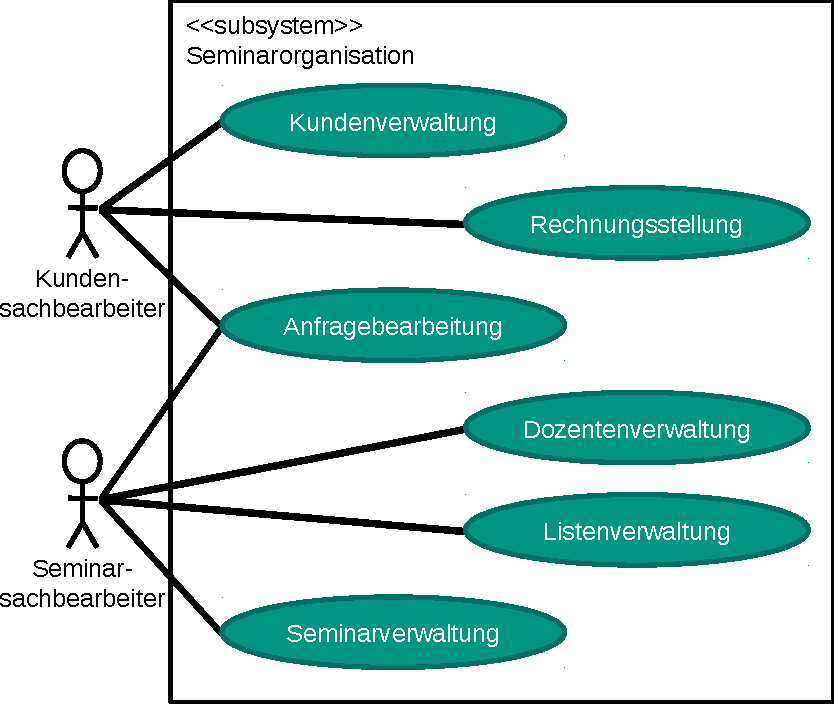
\includegraphics[width=0.8\textwidth]{szenario_seminarorganisation.pdf}
\end{center}

Akteure: Kundensachbearbeiter, Seminarsachbearbeiter.

Anwendungsfälle: Kundenverwaltung, Rechnungsstellung, Anfragebearbeitung, Dozentenverwaltung, Listenverwaltung, Seminarverwaltung.

Textuelle Beschreibung: (folgt)


\end{document}
